\documentclass[11pt,a5paper]{article}

\usepackage[T1]{fontenc}
\usepackage[utf8]{inputenc}
\usepackage{lmodern, microtype}
\usepackage[estonian]{babel}
\usepackage{siunitx}
\sisetup{inter-unit-product=\ensuremath{{}\cdot{}}, per-mode=fraction, exponent-product=\cdot, output-decimal-marker={,}}
\usepackage{graphicx}
\usepackage{wrapfig}
\usepackage{adjustbox}
\usepackage{tikz}
\usetikzlibrary{arrows.meta, patterns, patterns.meta}
\usepackage{pgfplots}
\usepackage[european]{circuitikz}
\tikzset{component/.style={draw,thick,circle,fill=white,minimum size=0.75cm,inner sep=0pt}}
\usepackage{amsmath,amssymb}
\usepackage{amsfonts}
\usepackage[hidelinks]{hyperref}
\usepackage{csquotes}
\usepackage{caption}
\usepackage{enumitem}
\topmargin=-3.0cm \textheight=19cm \textwidth=12.9cm
\oddsidemargin=-1.5cm  \evensidemargin=-1.5cm
\setlength{\parindent}{0pt} \setlength{\parskip}{6pt} \sloppy
\sloppy \relpenalty=10000 \binoppenalty=10000
\pagestyle{empty}

\newcommand{\numb}[1]{\vspace{5pt}\textbf{\large #1}}
\newcommand{\nimi}[1]{(\textsl{\small \uppercase{#1}})}
\newcommand{\punktid}[1]{(\emph{#1~p.})}
\newcounter{ylesanne}
\newcommand{\yl}[1]{\addtocounter{ylesanne}{1}\numb{\theylesanne.} \nimi{#1} \newblock{}}
\newcommand{\autor}[1]{}% Kasuta võistluse ajal
% \newcommand{\autor}[1]{\emph{Autor: #1}}% Kasuta kui vaja autorit

\begin{document}
\begin{center}
  \textbf{\Large Eesti koolinoorte 70. füüsikaolümpiaad} \par
  \emph{1. aprill 2023. a.\\Gümnaasiumi ülesanded (10.--12. klass)}
\end{center}

\resizebox{\textwidth}{!}{
  \emph{%
    \begin{tabular}{@{}l@{}}
      \textbf{Palun kirjutada iga ülesande lahendus eraldi lehele.}\\
      Lahendamisaeg on 5 tundi. \\
      Iga osavõtja võib lahendada kõiki pakutud ülesandeid. \\
      Arvesse lähevad 5 suurima punktide arvu saanud teoreetilist ja 1 eksperimentaalne ülesanne. \\
      Kasutada võib kirjutus- ja joonestusvahendeid ning kalkulaatorit. Muud abivahendid on keelatud.\\
      Eksperimentaalülesande lahendamisel võib kasutada üksnes loetelus toodud vahendeid. \\
      Mõõtemääramatuse hindamist ei nõuta.
    \end{tabular}
  }
} \par

\yl{SUJUV AUTOSÕIT}
Bussijuht tahab sõita sujuvalt, st et reisijatel, kes bussis püsti seisavad ja kusagilt kinni ei hoia, ei tekiks äkilise kiirendamise või pidurdamise tõttu tasakaalu kaotamise ja kukkumise ohtu. Seepärast suurendab ta pidurdades survet piduripedaalile tasapisi kuni bussi peatumiseni. Kas selline sõit on sujuv? Kui on sujuv, siis põhjendada, miks see nii on. Kui ei ole sujuv, siis selgitada, mis hetkel on seisvatel reisijatel oht tasakaal kaotada, mis suunas on neil oht kukkuda ning kuidas tuleks pidurdada, et pidurdamine oleks sujuv, st et seisvatel reisijatel ei tekiks kordagi ohtu tasakaalu kaotada?
\punktid{6} \autor{Jaan Kalda}

\yl{ELEKTRIKARJUS}
Elektrikarjusega karjatamisel ümbritseb karjamaad pikk traat, mis on postide abil maast elektriliselt isoleeritud. Elektrikarjuses olev generaator saadab sellesse traati impulsspinge: pingevabad perioodid vahelduvad lühikeste pingega perioodidega. Pingeimuplsi ajal võib elektrikarjuse pingegeneraatorit vaadelda kui elektromotoorjõudu $\mathcal E$, mis omab teatud sisetakistust $R$. Elektriimpulss on eluohtlik, kui inimest läbib vool, mis on suurem kui $I_0=\SI{30}{mA}$. Teatud marki elektrikarjuse kohta on teada järgmist: kui pingegeneraatori väljundklemmidest üks on maandatud ja teisest lähtuv karjaaia traat on maapinnast ideaalselt isoleeritud, siis traadi ja maapinna vaheline pinge on impulsi ajal $U_m=\SI{15}{kV}$. Inimene, kes kõnnib paljajalu ja on seetõttu heas elektrilises kontaktis maapinnaga, puudutab kuiva käega karjuse traati ning saab elektrilöögi. Eeldage, et inimese keha takistus on hulga väiksem, kui kuiva käenaha takistus $r=\SI 5\kohm$.\\
\osa Joonistage elektriskeem, mis kirjeldab olukorda, kui inimene saab parajasti karjuselt elektrilööki.\\
\osa Millised sisetakistuse $R$ väärtused on lubatavad?
\punktid{6} \autor{Jaan Kalda}

\newpage
\yl{LÄÄTS JA KAKS PEEGLIT}
Konstrueerige objekti $AB$ (vt joonist lisalehel) kõik kujutised. Skeemil on hall sein, sinine \SI{45}{\degree} kaldu poolläbilaskev peegel (pool valgusest läheb otse läbi, pool peegeldub nagu tavalises tasapeeglis), kumerlääts fookuskaugusega $f$ ja tasapeegel. Lahendage ülesanne lisalehel.
\punktid{8} \autor{Aigar Vaigu}

\yl{Laev}
Laev sõitis läbi Suessi kanali ning jäi sinna kinni nii, et blokeeris kogu kanali. Laeva pikkus on $l$, laius on $w$, kõrgus on $h$ ja mass on $m$. Veepiirist allpool on $k$ osa laeva ruumalast, kusjuures $klwh\rho < m$. Võib eeldada, et laev on ühtlase massijaotusega risttahukas ja $l \gg w$. Vee tihedus on $\rho$, raskuskiirendus $g$ ja kanali laius $d$. Hõõrdetegur laeva kere ja kanali vahel on $\mu$. Laeva mõlemat otsa tõmbavad puksiirlaevad kanali sihis eri suundades. Kui suure jõuga $F$ peavad puksiirlaevad tõmbama, et kinni jäänud laev hakkaks liikuma?
\punktid{8} \autor{Kaarel Kivisalu}

\yl{Sundventilatsioon}
Maril on kodus sundventilatsioon. Ta avastas, et ta peab õhuniisutit, mille paaki mahub $m=\SI{1}{\kg}$ vett, täitma iga kümne tunni tagant selleks, et hoida toas suhtelist õhuniiskust $r_1= 50 \%$. Väljas on temperatuur $T_2 = \SI{-5}{\celsius}$ ja suhteline õhuniiskus $r_2 = 80 \%$ ning toas on temperatuur $T_1= \SI{20}{\celsius}$. Kasutades juuresolevat küllastunud aururõhu graafikut, leidke mis kiirusega vahetab sundventilatsioon toas olevat õhku. Vee molaarmass on $M=\SI{18}{\gram\per\mole}$, gaasi universaalkonstant $R=\SI{8.31}{\joule\per\mole\per\kelvin}$ ja õhurõhk on $p=\SI{100}{\kilo\pascal}$.
\punktid{8} \autor{Kaur Aare Saar}
\begin{center}
  \vspace{-2em}
  \pgfkeys{/pgf/number format/.cd,1000 sep={}}% Suurtes arvudes komasid pole selguse huvides
  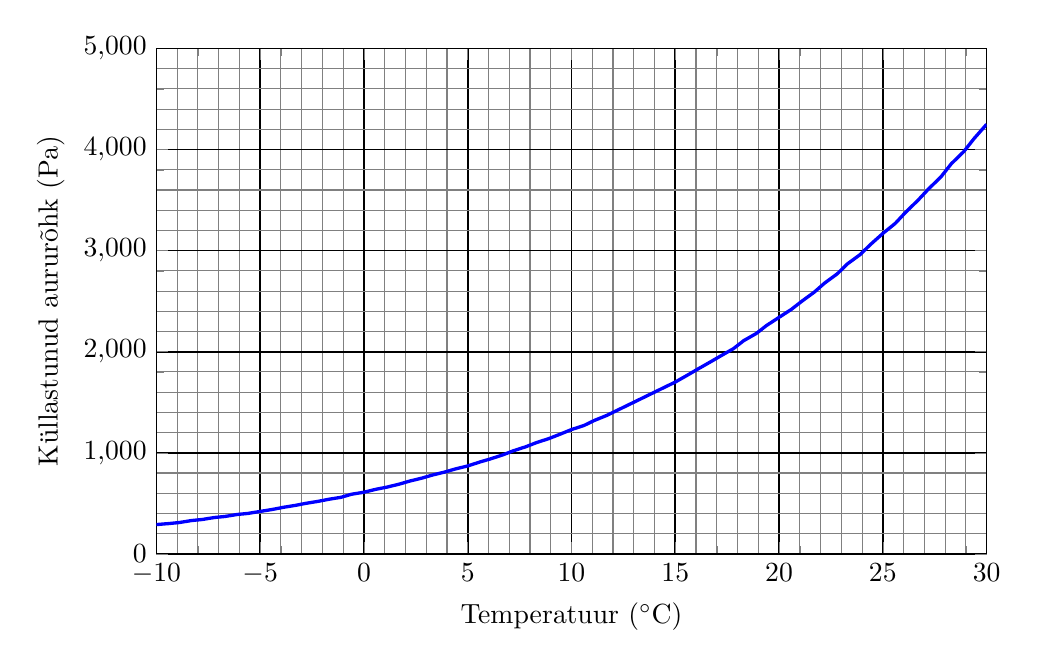
\begin{tikzpicture}
    \begin{axis}[
      xlabel={Temperatuur ($^\circ$C)},
      ylabel={Küllastunud aururõhk (Pa)},
      xmin=-10, xmax=30,
      ymin=0, ymax=5000,
      xtick={-10,-5,0,5,10,15,20,25,30},
      ytick={0,1000,2000,3000,4000,5000},
      minor tick num=4,
      grid=both,
      minor grid style={thin,gray},
      major grid style={semithick,black},
      width=\textwidth,
      height=8cm,
      ]

      \addplot[color=blue,very thick]
      coordinates {
        (-10.00,290.0)
        (-9.40,300.0)
        (-8.90,310.0)
        (-8.30,330.0)
        (-7.80,340.0)
        (-7.20,360.0)
        (-6.70,370.0)
        (-6.10,390.0)
        (-5.60,400.0)
        (-5.00,420.0)
        (-4.40,440.0)
        (-3.90,460.0)
        (-3.30,480.0)
        (-2.80,500.0)
        (-2.20,520.0)
        (-1.70,540.0)
        (-1.10,560.0)
        (-0.60,590.0)
        (0.00,610.0)
        (0.60,640.0)
        (1.10,660.0)
        (1.70,690.0)
        (2.20,720.0)
        (2.80,750.0)
        (3.30,780.0)
        (3.90,810.0)
        (4.40,840.0)
        (4.40,840.0)
        (5.00,870.0)
        (5.60,910.0)
        (6.10,940.0)
        (6.70,980.0)
        (7.20,1020.0)
        (7.80,1060.0)
        (8.30,1100.0)
        (8.90,1140.0)
        (9.40,1180.0)
        (10.00,1230.0)
        (10.60,1270.0)
        (11.10,1320.0)
        (11.70,1370.0)
        (12.20,1420.0)
        (12.80,1480.0)
        (13.30,1530.0)
        (13.90,1590.0)
        (14.40,1640.0)
        (15.00,1700.0)
        (15.60,1770.0)
        (16.10,1830.0)
        (16.70,1900.0)
        (17.20,1960.0)
        (17.80,2030.0)
        (18.30,2110.0)
        (18.90,2180.0)
        (19.40,2260.0)
        (20.00,2340.0)
        (20.60,2420.0)
        (21.10,2500.0)
        (21.70,2590.0)
        (22.20,2680.0)
        (22.80,2770.0)
        (23.30,2870.0)
        (23.90,2960.0)
        (24.40,3060.0)
        (25.00,3170.0)
        (25.60,3270.0)
        (26.10,3380.0)
        (26.70,3500.0)
        (27.20,3610.0)
        (27.80,3730.0)
        (28.30,3860.0)
        (28.90,3980.0)
        (29.40,4110.0)
        (30.00,4250.0)
      };
    \end{axis}
  \end{tikzpicture}
  \vspace{-3em}
\end{center}

\yl{Nõel vees}
Nõel massiga $m=\SI{0.5}{\g}$ ning pikkusega $l=\SI{6}{\cm}$ asetatakse aeglaselt vee pinnale. Millise nurga alla on veepind nõela juures horisontaalpinna suhtes paindunud? Vee pindpinevustegur $\sigma=\SI{72.8}{\mN\per\m}$ ja raskuskiirendus $g=\SI{9.81}{\m\per\s\squared}$. Üleslükkejõuga võib mitte arvestada.
\punktid{10} \autor{Martne Rannut}

\yl{TEHISKAASLANE} Tehiskaaslane tiirleb ümber planeedi ringorbiidil raadiusega $r=\SI{55199}{\km}$ kiirusega $v=\SI{2.4}{\km\per\s}$. Tehiskaaslasele on lühikese aja jooksul võimalik anda kiiruse muut $\Delta v=\SI{0.7}{\km\per\s}$.
\\a) Mis oleks tehiskaaslase suurim kaugus planeedi keskmest $R_1$, kui tehiskaaslasele antaks kiirendus selle liikumissuunas?
\\b) Mis oleks suurim kaugus $R_2$, kui kiirenduse suund oleks planeedist eemale?
\punktid{10} \autor{Eero Vaher}

\yl{Kuulitõuge}
Nagu mehaanikast hästi teada, lendab visatud keha antud algkiiruse juures (õhutakistuse puudumisel) kõige kaugemale siis, kui viskenurk horisontaali suhtes on \ang{45}. Kuulitõukespordis on optimaalne nurk mõnevõrra väiksem.
\\a) Leidke selle väärtus, eeldades et kuuli maksimaalne lennukaugus on $s_\text{m}=\SI{20}{m}$, tõukaja vabastab kuuli maapinnast kõrgusel $h_0=\SI{2}{m}$ ja algkiirus ei sõltu tõukesuunast.
\\b) Kui suur on sellise kuuli algkiirus?
\\Raskuskiirendus $g=\SI{9.8}{\meter\per\second\squared}$.
\punktid{10} \autor{Valter Kiisk}

\yl{Staatiline elekter}
A4 formaadis kile kogupindalaga $S= \SI{630}{\square\cm}$ on laetud ühtlase positiivse pindtihedusega staatilise elektriga. Kui see kile asetada vastu  maandatud metallplaati, mille pindala on kile omast hulga suurem, siis \enquote{kleepub} kile vastu plaati ning selleks, et libistada kilet mööda plaati, on vaja rakendada jõudu $F=\SI{0.1}{\N}$ plaadi sihis; hõõrdetegur kile ja plaadi vahel on $\mu=\num{0.5}$. Kile mass on hulga väiksem kui \SI{20}{\g}. Millise pinge omandab kile metallplaadi suhtes, kui see tõmmata plaadilt lahti ning hoida plaadist kaugusel $h=\SI{5}{\cm}$, paralleelselt plaadiga? Elektriline konstant $\varepsilon_0=\SI{8.85e-12}{\F\per\m}$.
\punktid{12} \autor{Jaan Kalda}

\yl{Uppuv pall}
Vees ujub vettinud ja vett täis tennisepall nii, et see on peaaegu üleni vee all ning ülemine serv puudutab veepinda. Kaldalt, $H=\SI 2\m$ kõrguselt vaadates näib, et pall on ellipsoidi kujuliselt lapik, kusjuures laiuse ja kõrguse suhe on $k=3$. Kui kaugel vaataja silmast on pall, kui vee murdumisnäitaja $n=\frac 43$? Ülesande lahendamisel võib teha mõistlikke lähendusi.
\punktid{12} \autor{Jaan Kalda}

\end{document}